\documentclass[tikz,border=2pt,png]{standalone}
\usepackage{tkz-euclide}
\usetkzobj{all}

\begin{document}
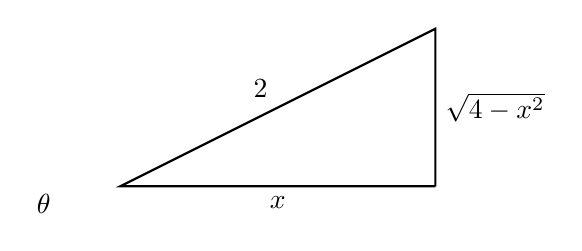
\begin{tikzpicture}[thick]
\draw(0,0) -- (90:2cm) node[midway,right]{$\sqrt{4-x^2}$} -- (0:-4cm)
node[midway,above left]{$2$} -- (0,0)
node[midway,below]{$x$};
\coordinate (A) at (-4cm,0);
\coordinate (B) at (0cm,0cm);
\coordinate (C) at (0cm,2cm);
\tkzLabelAngle[pos = 1](C,A,B){$\theta$};
\end{tikzpicture}
\end{document}

%%% Local Variables:
%%% mode: latex
%%% TeX-master: t
%%% End:
